\documentclass[a4paper,oneside]{memoir}
\usepackage[T1]{fontenc}
\usepackage[utf8]{inputenc}
\usepackage[english]{babel}


\usepackage[format=hang]{caption,subfig}
\usepackage{graphicx}
\usepackage{pdflscape} % Gør landscape-environmentet tilgængeligt
\usepackage[draft]{fixme}     % Indsæt "fixme" noter i drafts.
\usepackage{hyperref}  % Indsæter links (interne og eksterne) i PDF


\renewcommand{\ttdefault}{pcr} % Bedre typewriter font
%\usepackage[sc]{mathpazo}     % Palatino font
\renewcommand{\rmdefault}{ugm} % Garamond
\usepackage[garamond]{mathdesign}

%\overfullrule=5pt
%\setsecnumdepth{part}
\setcounter{secnumdepth}{-1} % Sæt overskriftsnummereringsdybde. Disable = -1.

\newcommand{\EDSL}{EDSL (Embedded Domain Specific Language) \renewcommand{\EDSL}{ EDSL }}
\hyphenation{da-ta-be-hand-ling}
\hyphenation{pro-gram-me-rings-sprog-et}
\hyphenation{brug-es}

\title{Synopsis}

\author{Johan Brinch (Zerrez@gmail.com), \\
Morten Brøns-Pedersen (mortenbp@gmail.com) \\ og
Jesper Reenberg (jesper.reenberg@gmail.com)}




\date{\today}
\pagestyle{plain}



\begin{document}
\maketitle

\section{Project title}

``Skal vi lege Dr.''

\section{Project definition}

Programs written in declarative programming languages has a wide veracity of
advantages that makes them specially souted for quick and correct statical
analysis.

\fixme{hvilke?}

The purpose of this project is to take advantages of the above to do semi
automatic refactoring of the source code by means of different hard coded
plugins. One of the simplest plugins would do renaming of variable and function
names based on scope. This can then be extended to another plugin that given two
finite sets P (``patterns'') and C (``code'') of function definitions will
return a series of propositions for refactoring the code C. Such a proposition
is a set, F, of declarations such that a subset of F has the same signature as
C but to more extend uses declarations that shares syntax tree with declarations
from P.



\fixme{bør andre typer plugins nævnes? Disse kan jo evt blot pilles væk i
  afgrænsningen}




\begin{quotation}
  Programmer i deklarative programmeringssprog har en række fordele, som gør dem
  særdeles velegnet til hurtig og korrekt statisk analyse.

  Formålet med denne opgave er at udnytte ovenstående til at foretage
  halvautomatiske refaktoreringer, som kun vanskeligt kan benyttes (eller
  sjældent er relevante) i øvrige sprog.
\end{quotation}

\section{Elaboration}

\subsection{Motivation}

The target audience for this tool is novice programmers in functional
programming languages which is not used to work with the programming patterns
and -templates from this paradime. 

\begin{quotation}
  Målgruppen for det udviklede værktøj er novicer i funktionsprogrammering, som
  ikke er vant til at benytte de særlige programmeringsmønstre og -skabeloner
  fra dette paradigme.
\end{quotation}



\subsection{Implementation}


\begin{itemize}
\item Datastrukturer i flow ned igennem, skal bygge videre og ikke smide noget
  data væk.

\item Al kommunikation mellem frontend og server sker igennem JSON via IO.

\item Plugins skal kompiles med. (Alle plugins skal være slukket fra start)


\item Der kan tænkes flere forskellige SML parser niveauer 
  \begin{itemize}

  \item Der skal derfor indføres "runlevels". Så ved hvert parsnings afslut skal
    de plugin spawnes som "hooker" dette parsetræ (evt. kun 1 tråd der efter tur
    eksekverer alle plugins som hooker den givne level), samtidig med at der
    spawnes en tråd til at lave næste parsnings niveau.
  \end{itemize}
\end{itemize}

\section{Learning objectives}

\begin{enumerate}
\item 
\end{enumerate}

\section{Afgrænsninger}


\begin{enumerate}
\item There will not be developed a \textit{.CM}-file parser to the
  \texttt{Source Description} interface.

\item The \texttt{SML Parser} will not handle syntax errors. 
\end{enumerate}


\section{Task's}

\begin{enumerate}
\item Design the \texttt{Source Description} API. (1 week)

\item Implement a \textit{.MLB}-file parser (\texttt{MLB Parser}) from the MLB
  definition (1 week) 
\url{http://www.itu.dk/research/mlkit/index.php/ML_Basis_Files}

\item Design the concrete syntax tree to be used by the \texttt{SML
    Parser}. This needs to be done correct the first time. (1 week)

\item Create the \texttt{SML Parser} (3 weeks).

\item Create the \texttt{Refactoring Plugin} (3 weeks).

\item Create the \texttt{SMLserver} (1 week).
  \begin{itemize}
  \item Connect the \texttt{SML Parser} and \texttt{Refactoring Plugin} using threads
  \end{itemize}

\item Create the missing links in the \texttt{SMLserver} (2 weeks)
  \begin{itemize}
  \item Create the \texttt{non project files parser}\footnote{correct to the
      right name} and connect it with the \texttt{MLB Parser} into the
    \texttt{Source Description}.

  \item Create the \texttt{Project Manager}.

  \item Connect the \texttt{Source Description} with the \texttt{Project
      Manager}.

  \item Connect the \texttt{Project Manager} with the \texttt{SML Parser}.
  \end{itemize}

\item Create the \texttt{Communication Interface} between the \texttt{SMLserver}
  and the front end
  \begin{itemize}
  \item Create a plugin to the front end that will support the
    \texttt{Communication Interface}.
  \end{itemize}
\end{enumerate}

\section{Expansion (``nice to have'')}


\begin{enumerate}
\item A incremental \texttt{SML Parser}

\item That the \texttt{SML Parser} can handle syntax errors. I.e. by skipping
  the source code until next valid expression and then continue to parse. The
  skipped part could be reported to then front end and then handled approprietly
  (e.g., underlined).

\item Support of \texttt{DocString} by the \texttt{Communication Bridge} so when
  the front end hovers a function call it can show the \texttt{DocString}
  describing parameters and what the function does.
\end{enumerate}


\appendix

\chapter{Timetable}

\fixme{her kommer en tidstabel}

\chapter{Flow diagram}

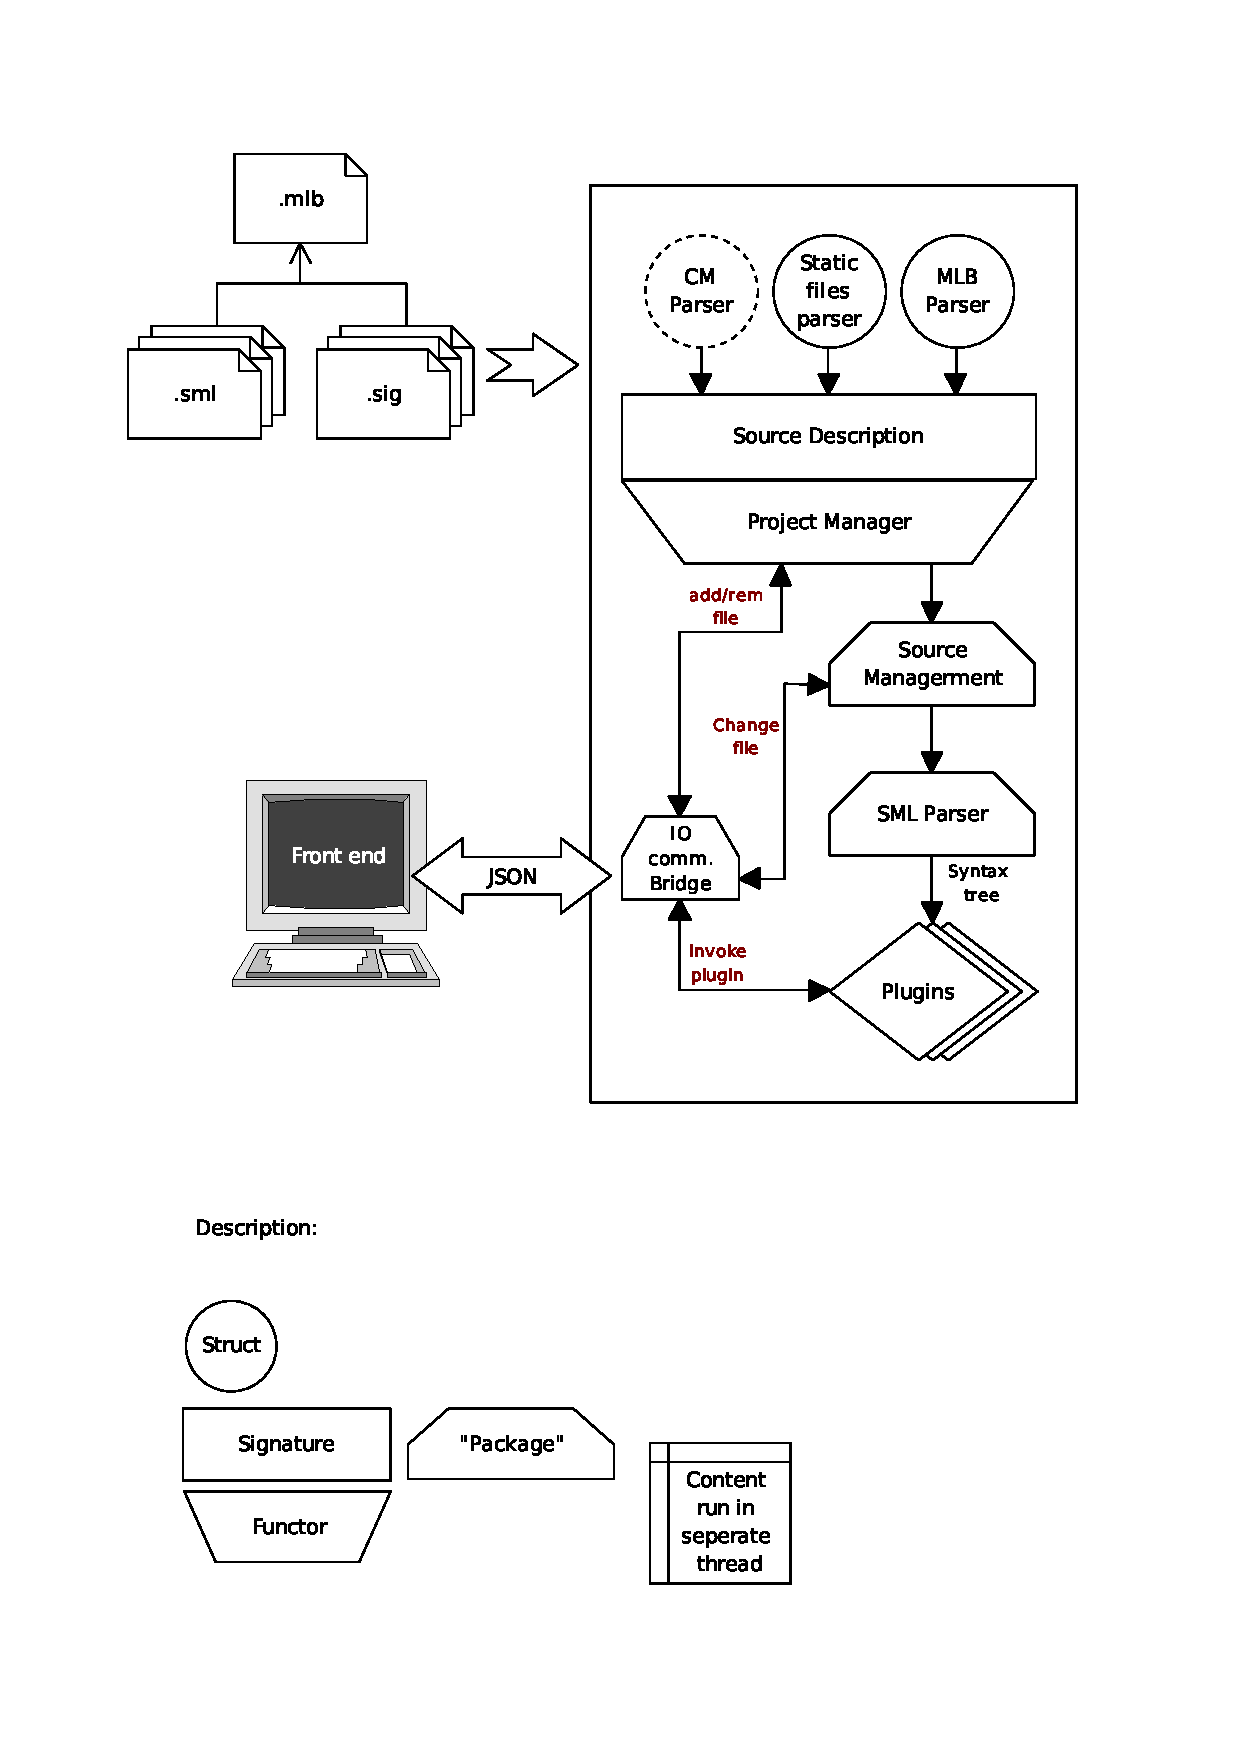
\includegraphics[width=\textwidth-1]{../drawings/flow}



%\bibliographystyle{plain}
%\bibliography{synopsis}

\end{document}

%%% Local Variables: 
%%% mode: latex
%%% TeX-master: t
%%% End: 
